\hypertarget{scala-types}{%
\section{Scala - Types}\label{scala-types}}

\begin{figure}[H]
\centering
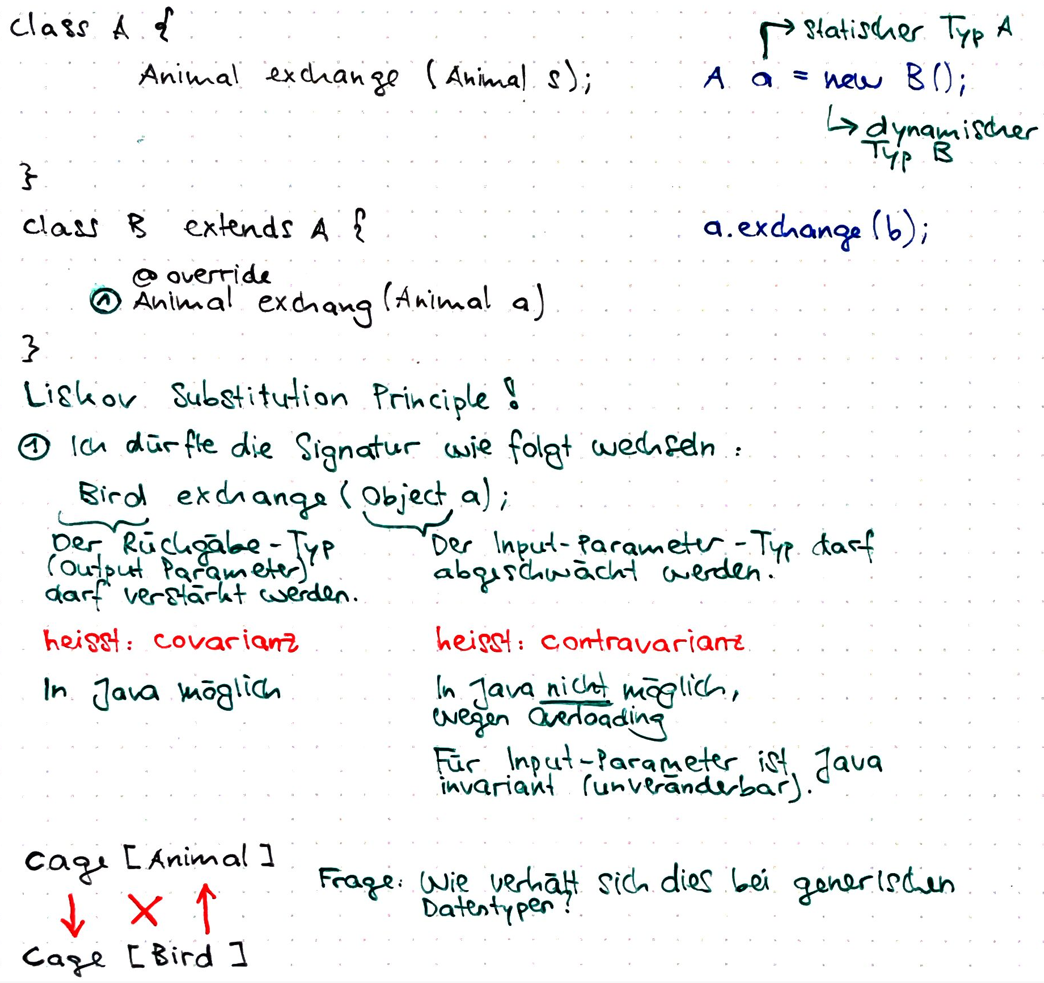
\includegraphics[width=0.85\textwidth]{figures/scalaVarianceIntro.png}
\caption{Variance Introduction}
\end{figure}

\hypertarget{parameterized-types}{%
\subsection{Parameterized Types}\label{parameterized-types}}

\hypertarget{generic-classes}{%
\subsubsection{Generic Classes}\label{generic-classes}}

\begin{lstlisting}[language=scala,mathescape=false]
case class Pair[T, S](val first: T, val second: S)

scala> val p1 = Pair(42, "String")
p1: Pair[Int,String] = Pair@4c5853eb
\end{lstlisting}

\hypertarget{generic-functions}{%
\subsubsection{Generic Functions}\label{generic-functions}}

\begin{lstlisting}[language=scala,mathescape=false]
def getMiddle[T](a: Array[T]) = a(a.length / 2)

scala> getMiddle(Array("one", "two", "three"))
res1: String = two
scala> getMiddle(Array(1, "two"))
res2: Any = two
\end{lstlisting}

\hypertarget{type-variable-bounds}{%
\subsubsection{Type Variable Bounds}\label{type-variable-bounds}}

\textbf{Upper Bounds}

\begin{lstlisting}[language=scala,mathescape=false]
case class Pair[T <: Comparable[T]](val p1: T, val p2: T) {
    def smaller = if(p1.compareTo(p2) < 0) p1 else p2
}

scala> val p = Pair("Stan", "Ollie")
p: Pair[String] = Pair(Stan,Ollie)
scala> p.smaller
res10: String = Ollie
scala> Pair(List("one"), List("two"))
error: inferred type arguments [List[String]] do not conform to class Pair's type parameter bounds [T <: Comparable[T]] new Pair(List("one"), List("two"))
\end{lstlisting}

This throws an error, since Lists do not implement Comparable.

\textbf{Lower Bounds}

\begin{lstlisting}[language=scala,mathescape=false]
case class Pair[T](val p1: T, val p2: T) {
    def setFirst(newP1: T) = new Pair[T](newP1, p2)
}

scala> val p = Pair("one", "two")
p: Pair[String] = Pair(one,two)
scala> p.setFirst(1)
<console>:13: error: type mismatch;
found    : Int(1)
required : String
            p.setFirst(1)
\end{lstlisting}

Since Pair is immutable, a new instance has to be created. With the
above definition, the resulting pair (when calling setFirst) is always
of the same type, even if something more general is added.

\begin{lstlisting}[language=scala,mathescape=false]
case class Pair[T](val p1: T, val p2: T) {
    def setFirst[R >: T](newP1: R) = new Pair[R](newP1, p2)
}

scala> val p = Pair("one", "two")
p: Pair[String] = Pair(one,two)
scala> p.setFirst(1)
res1: Pair[Any] = Pair(1,two)
scala> p.setFirst(null)
res2: Pair[String] = Pair(null,two)
\end{lstlisting}

The replacement type for the type variable of the new pair must be a
supertype of the pair's component type T

\hypertarget{bounds}{%
\subsubsection{Bounds}\label{bounds}}

Multiple lower and upper bounds can be specified with a compound type

\begin{lstlisting}[language=scala,mathescape=false]
def foo[T <: Comparable[T] with Serializable](x: T) = x
\end{lstlisting}

A type variable can have both an upper and a lower bound

\begin{lstlisting}[language=scala,mathescape=false]
// T >: Lower <: Upper
scala> class MBounds[T >: String <: AnyRef]
scala> new MBounds[String]
res1: MBounds[String] = MBounds@5fc59667
scala> new MBounds[CharSequence]
res2: MBounds[CharSequence] = MBounds@794579f3
scala> new MBounds[AnyRef]
res3: MBounds[AnyRef] = MBounds@4f028abf
\end{lstlisting}

\hypertarget{variance}{%
\subsection{Variance}\label{variance}}

It depends on the situation, which variance should apply or not.

\begin{figure}[H]
\centering
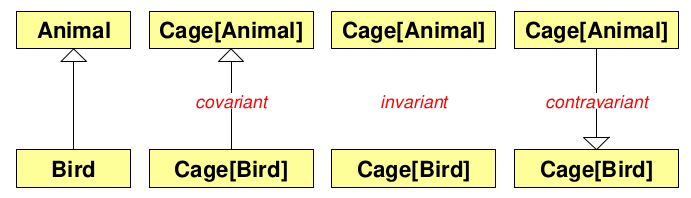
\includegraphics[width=0.7\textwidth]{figures/coAndContravarianz.png}
\caption{Variance}
\end{figure}

\begin{itemize}
\tightlist
\item
  If I only read from the object I receive, then the object need to be
  covariant (like output parameter)
\item
  If I only write to the object I receive, then the object need to be
  contravariant (like input parameter)
\item
  If I read and write from and to the object, the object needs to be
  invariant
\end{itemize}

\hypertarget{variance-in-java}{%
\subsubsection{Variance in Java}\label{variance-in-java}}

In Java, generic types are basically invariant, but you are able to
specify covariance or contravariance with super or extends.

Generics:

\begin{lstlisting}[language=scala,mathescape=false]
public class Test1 {
    static class Animal {}
    static class Bird extends Animal {}
    static class Cage<T> {}
    public static void main(String[] args) {
        Cage<Bird> birdCage = new Cage<Bird>();
        Cage<Animal> animalCage;
        animalCage = birdCage;
    }
}

//Compiler Error: Type mismatch:
//cannot convert from Cage<Bird> to Cage<Animal>
\end{lstlisting}

Arrays:

\begin{lstlisting}[language=scala,mathescape=false]
public class Test2 {
    static class Animal {}
    static class Bird extends Animal {}
    public static void main(String[] args) {
        Bird[] birdCage = new Bird[1];
        Animal[] animalCage = birdCage;
        animalCage[0] = new Animal();
    }
}

//Runtime Error: Exception in thread "main"
//java.lang.ArrayStoreException: Test2$Animal
//at Test2.main(Test2.java:12)
\end{lstlisting}

Wird auf ein Element im Array zugegriffen, wird jedes mal geprüft ob es
sich beim aktuellen Element um den dynamischen Typ des Arrays handelt
(und nicht um den statischen Typs).

\hypertarget{variance-in-scala}{%
\subsubsection{Variance in Scala}\label{variance-in-scala}}

\textbf{\textit{Read-only (immutable) =\textgreater{} covariant}}\\
A bird cage can be considered as a special animal cage (as it also
contains an animal =\textgreater{} expectation met!)

\textbf{\textit{Write-only =\textgreater{} contravariant}}\\
An animal cage can be considered a special bird cage (as it can be used
to put birds in it =\textgreater{} expectation met!)

\begin{lstlisting}[language=scala,mathescape=false]
scala> class Animal; class Bird extends Animal
scala> class Cage[A]
scala> val animalCage: Cage[Animal] = new Cage[Bird]
<console>:14: error: type mismatch;
found: Cage[Bird]
required: Cage[Animal]
Note: Bird <: Animal, but class Cage is invariant in type A.
You may wish to define A as +A instead. (SLS 4.5)

scala> val birdCage: Cage[Bird] = new Cage[Animal]
<console>:14: error: type mismatch;
found: Cage[Animal]
required: Cage[Bird]
Note: Animal >: Bird, but class Cage is invariant in type A.
You may wish to define A as -A instead. (SLS 4.5)
\end{lstlisting}

\textbf{Covariance} 

Use + to declare a covariant type parameter

\begin{lstlisting}[language=scala,mathescape=false]
scala> class Animal; class Bird extends Animal
scala> class Cage[+A]

scala> val animalCage: Cage[Animal] = new Cage[Bird]
animalCage: Cage[Animal] = Cage@62d75a88

scala> val birdCage: Cage[Bird] = new Cage[Animal]
<console>:14: error: type mismatch;
\end{lstlisting}

\textbf{Contravariant}

Use - to declare a contravariant type parameter

\begin{lstlisting}[language=scala,mathescape=false]
scala> class Animal; class Bird extends Animal
scala> class Cage[-A]

scala> val animalCage: Cage[Animal] = new Cage[Bird]
<console>:14: error: type mismatch;

scala> val birdCage: Cage[Bird] = new Cage[Animal]
birdCage: Cage[Bird] = Cage@1bdab192
\end{lstlisting}

\textbf{Drawbacks}

When can we use variance declarations on class type params?\\
The answer depends on whether type variables are used in producer
(positive) or consumer (negative) positions

\begin{itemize}
\tightlist
\item
  To be safe for covariance, a type parameter T must appear only in
  ``producer'' (positive) positions in method signatures
\item
  To be safe for contravariance, a type parameter T must appear only in
  ``consumer'' (negative) positions in method signatures
\end{itemize}

\begin{lstlisting}[language=scala,mathescape=false]
abstract class Cage [A] {
    def get: A              //+
    def put(a: A): Unit     //-
    val animal: A           //+ (because immutable)
    var animal2: A          //+-
}
\end{lstlisting}

The Scala compilers throws an error if these rules are harmed.

\textbf{Variance Declarations and Subclassing}

\begin{lstlisting}[language=scala,mathescape=false]
class Cage[A] // invariant
class SpecialCage[+A] extends Cage[A] // not ok
class SpecialCage[ A] extends Cage[A] // ok
class SpecialCage[-A] extends Cage[A] // not ok

class Cage[+A] // covariant
class SpecialCage[+A] extends Cage[A] // ok
class SpecialCage[ A] extends Cage[A] // ok
class SpecialCage[-A] extends Cage[A] // not ok

class Cage[-A] // contravariant
class SpecialCage[+A] extends Cage[A] // not ok
class SpecialCage[ A] extends Cage[A] // ok
class SpecialCage[-A] extends Cage[A] // ok
\end{lstlisting}

\hypertarget{variance-in-java-bounded-wildcards}{%
\subsubsection{Variance in Java: Bounded
Wildcards}\label{variance-in-java-bounded-wildcards}}

Java controls variance on use-site (not on declaration site)

\begin{lstlisting}[language=scala,mathescape=false]
//Covariance
void readAnimal(Cage<? extends Animal> cage) {
    Animal a = cage.getContent();
}
//One can only read from the cage

//Contravariance
void storeBird(Bird b, Cage<? super Bird> cage) {
    cage.setContent(b);
}
//One can't read anymore. 
//On the parameter cage, only methods can be invoked which have the type parameter in a contravariant position
\end{lstlisting}

\clearpage
\textbf{Example}

\begin{lstlisting}[language=scala,mathescape=false]
class A {}
class B extends A {}
class C extends B {}
class Cage<T extends A> {
    private T x;
    public T getContent() { return x; }
    public void setContent(T a) { x = a; }
    public T replaceContent(T a) { T ret = x; x = a; return ret; }
}

public static void readContent(Cage<? extends B> cage) {
    B b = cage.getContent();
    // cage.setContent(new B()); // method not applicable
    // a = cage.replaceContent(new B());
    cage.setContent(null);
    b = cage.replaceContent(null);
}

public static void writeContent(Cage<? super B> cage) {
    // B b = cage.getContent();
    // type mismatch
    cage.setContent(new B());
    // b = cage.replaceContent(new B()); // type mismatch
}
\end{lstlisting}

\hypertarget{problems}{%
\paragraph{Problems}\label{problems}}

\begin{itemize}
\tightlist
\item
  Types on use-site can get complicated, with nesting of variance
  annotations
\item
  Annotations must be maintained on every use of a generic type
\end{itemize}

\hypertarget{comments}{%
\paragraph{Comments}\label{comments}}

\begin{itemize}
\tightlist
\item
  Declaration-site variance is the choice if the language prefers
  immutable data structures
\item
  Use-site variance is just right for mutable (invariant) data
  structures. It gives each service the choice which variance, if any,
  is appropriate
\end{itemize}

\clearpage